\documentclass{article}

\title{Laboratorio - Esercizio con Ladder}
\author{Benedetta Vitale ed Emilio Meroni}
\date{5 maggio 2024}

\usepackage{tabularx} %per le tabelle
\usepackage[italian]{babel}  % Lingua
\usepackage{booktabs} %per le linee
\usepackage{graphicx} %per le immagini
\usepackage{pdfpages} %include pdf
\usepackage{float}

\begin{document}

\maketitle

\tableofcontents

\section{Introduzione}

\begin{figure}[b]
    \centering
    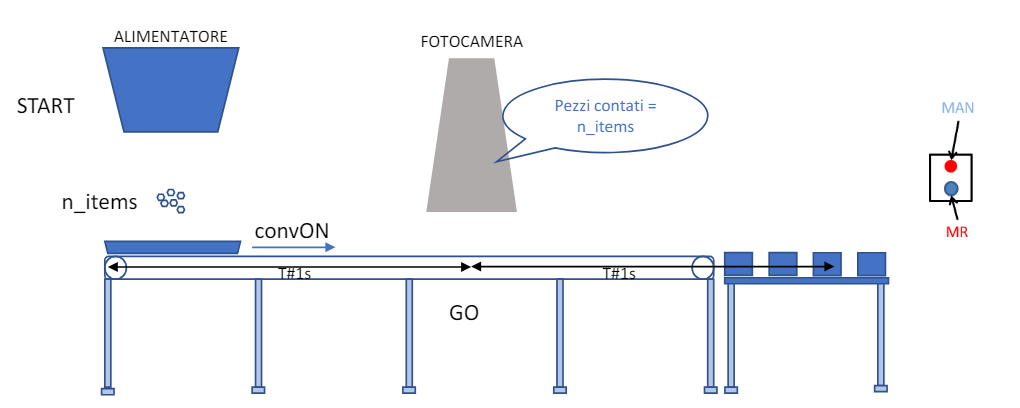
\includegraphics[width = 0.8 \linewidth]{schematico.png}
    \caption{Schematico del sitema}
    \label{fig:schematico}
\end{figure}

Il sistema che si deve gestire serve per controllare se è presente il numero corretto di pezzi (10 pz) in un kit.
\\

Per avviare il ciclo di lavoro si parte dalla pressione di un pulsate \textit{START}, ma se è necessario fare manutenzione oppure è già in corso un'altro ciclo, la pressione del tasto viene inibita.
\\

All'avvio del ciclo un \textit{alimentatore} [Fig:\ref*{fig:schematico}] eroga un numero di pezzi(\textit{n\_items}), prossimo a 10 pz, in una vaschetta che viaggerà per un secondo fino a fermarsi al di sotto di una fotocamera. Essa serve per rilevare il numero di \textit{n\_items} inseriti; e, se sono uguali a dieci (\textit{n\_kit}), il nastro trasportatore si avvierà ancora per un secondo fino al raggiungere la parte di assemblaggio dei kit. Mentre se il numero di pezzi rilevati è diverso da \textit{n\_kit}, il sistema si blocca in attesa dell'intervento dell'operatore. Una volta che i pezzi all'interno della vaschetta saranno nuovamente dieci, il nastro trasportatore si avvierà per un seconodo.
\\

Si devono contare il numero di volte che i pezzi inseriti dall'\textit{alimentatore} siano pari a \textit{n\_kit}, inoltre il sistema andrà in manutenzione dopo dieci cilci di lavoro.

\section{Definizione Variabili}
In questa sezione verranno definite e spiegate le diverse variabili che utilizzeremo, saranno sezionate per categoria:
\begin{itemize}
    \item Input e Output
    \item Stati
    \item Valori e Costanti
\end{itemize}

\subsection{Input e Output del sistema}
\begin{center}
    \begin{tabular}{l l l l }
        \toprule
        \textbf{Nome}  & \textbf{Tipologia} & \textbf{Descrizione}                           \\
        \midrule
        \midrule
        CONVon         & Output             & Motore del nastro trasportatore                \\
        \midrule

        START          & Input              & Avvio del ciclo di lavoro                      \\
        \midrule

        GO             & Input              & Pulstante per riprendere il ciclo dopo lo stop \\
                       &                    & indotto dal numero sbagliato di pezzi          \\
        \midrule
        MR             & Input              & Reset della manutenzione                       \\
        \midrule
        RESET\_COUNTER & Input              & Pulsante per resettare il conteggio dei pezzi  \\
                       &                    & buoni                                          \\
        \bottomrule
    \end{tabular}
\end{center}


\subsection{Stati del sistema}
\begin{center}
    \begin{tabular}{l l}
        \toprule
        \textbf{Nome}  & \textbf{Descrizione}                                       \\
        \midrule
        \midrule

        ON             & Identifica che il ciclo è attivo                           \\
        \midrule
        MUOVI          & Identifica lo stato del nastro trasportatore attivo        \\
        \midrule
        FOTOCAMERA     & Stato in cui la fotocamera sta leggendo i dati             \\
        \midrule
        RISULTATI      & Indichiamo che stiamo confrontando i dati della fotocamera \\
        \midrule
        BUONO          & Quando i pezzi contati sono pari a n\_kit                  \\
        \midrule
        NON\_BUONO     & Quando i pezzi contati sono diversi da n\_kit              \\
        \midrule
        ATTESA\_UTENTE & Quando si aspetta l'intervento dell'operatore              \\
        \midrule
        MAN            & Stato di manutenzione                                      \\

        \bottomrule
    \end{tabular}
\end{center}

\subsection{Valori e Costanti}
\begin{center}
    \begin{tabular}{l l c l}
        \toprule
        \textbf{Nome} & \textbf{Tipo} & \textbf{Valore Predefinito} & \textbf{Descrizione}                   \\
        \midrule
        \midrule

        n\_corrette   & INT           & 10                          & Numero di volte che la fotocamera ha   \\
                      &               &                             & letto n\_kit  oggetti                  \\
        \midrule

        n\_items      & INT           & -                           & Numero di oggetti nella vaschetta      \\
        \midrule

        n\_kit        & INT           & 10                          & Valore degli item necessari nel kit    \\
        \midrule
        n\_cicli\_man & INT           & 10                          & Numero dei cicli prima che andiamo \\
                      &               &                             & in manutenzione                        \\
        \midrule

        tFotocamera   & TIME          & T\#500ms                    & Tempo che la fotocamera impiega per    \\
                      &               &                             & leggere i dati                         \\
        \midrule
        t1s           & TIME          & T\#1s                       & Tempo 1 secondo                        \\

        \bottomrule
    \end{tabular}
\end{center}

\section{Come abbiamo lavorato}
Per questo lavoro utilizziamo uno schema a \textit{stati}, principalmente perché il sistema si presenta molto bene per questo metodo, inoltre è venuto più facile a pensarlo in questo modo.
\\

Oltre alle variabili date dal testo, e quelle degli stati, abbiamo deciso di aggiungere una fase in più alla lettura della fotocamera, simulado con $500ms$ il tempo per effettuare il conteggio.
Inoltre, abbiamo scelto di inserire delle variabili aggiuntive per avere più controllo durante il debug del programma, in particolare sono:
\begin{itemize}
    \item \textit{t1s}: variabile che indica un secondo per il nastro trasportatore; utilizzata per rallentare il sistema e verificarne la correttezza degli stati in quel momento.
    \item \textit{n\_cicli\_man}: variabile che indica il numero di cicli prima di andare in manutenzione (normalmente settata a dieci), in debug abbassata a due/tre cicli di lavoro.
\end{itemize}

In figura \ref*{fig:schema} presentiamo uno schema che rappresenta gli stati del sistema.
\begin{figure}[H]
    \centering
    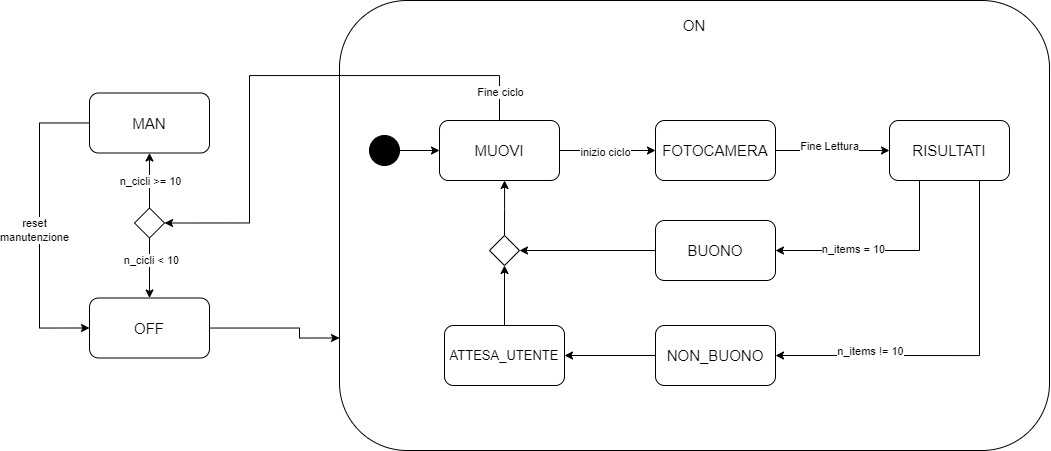
\includegraphics[width = 1\linewidth]{Diagramma_Stati.png}
    \caption{diagramma degli stati}
    \label{fig:schema}
\end{figure}


\section{Programma Ladder}
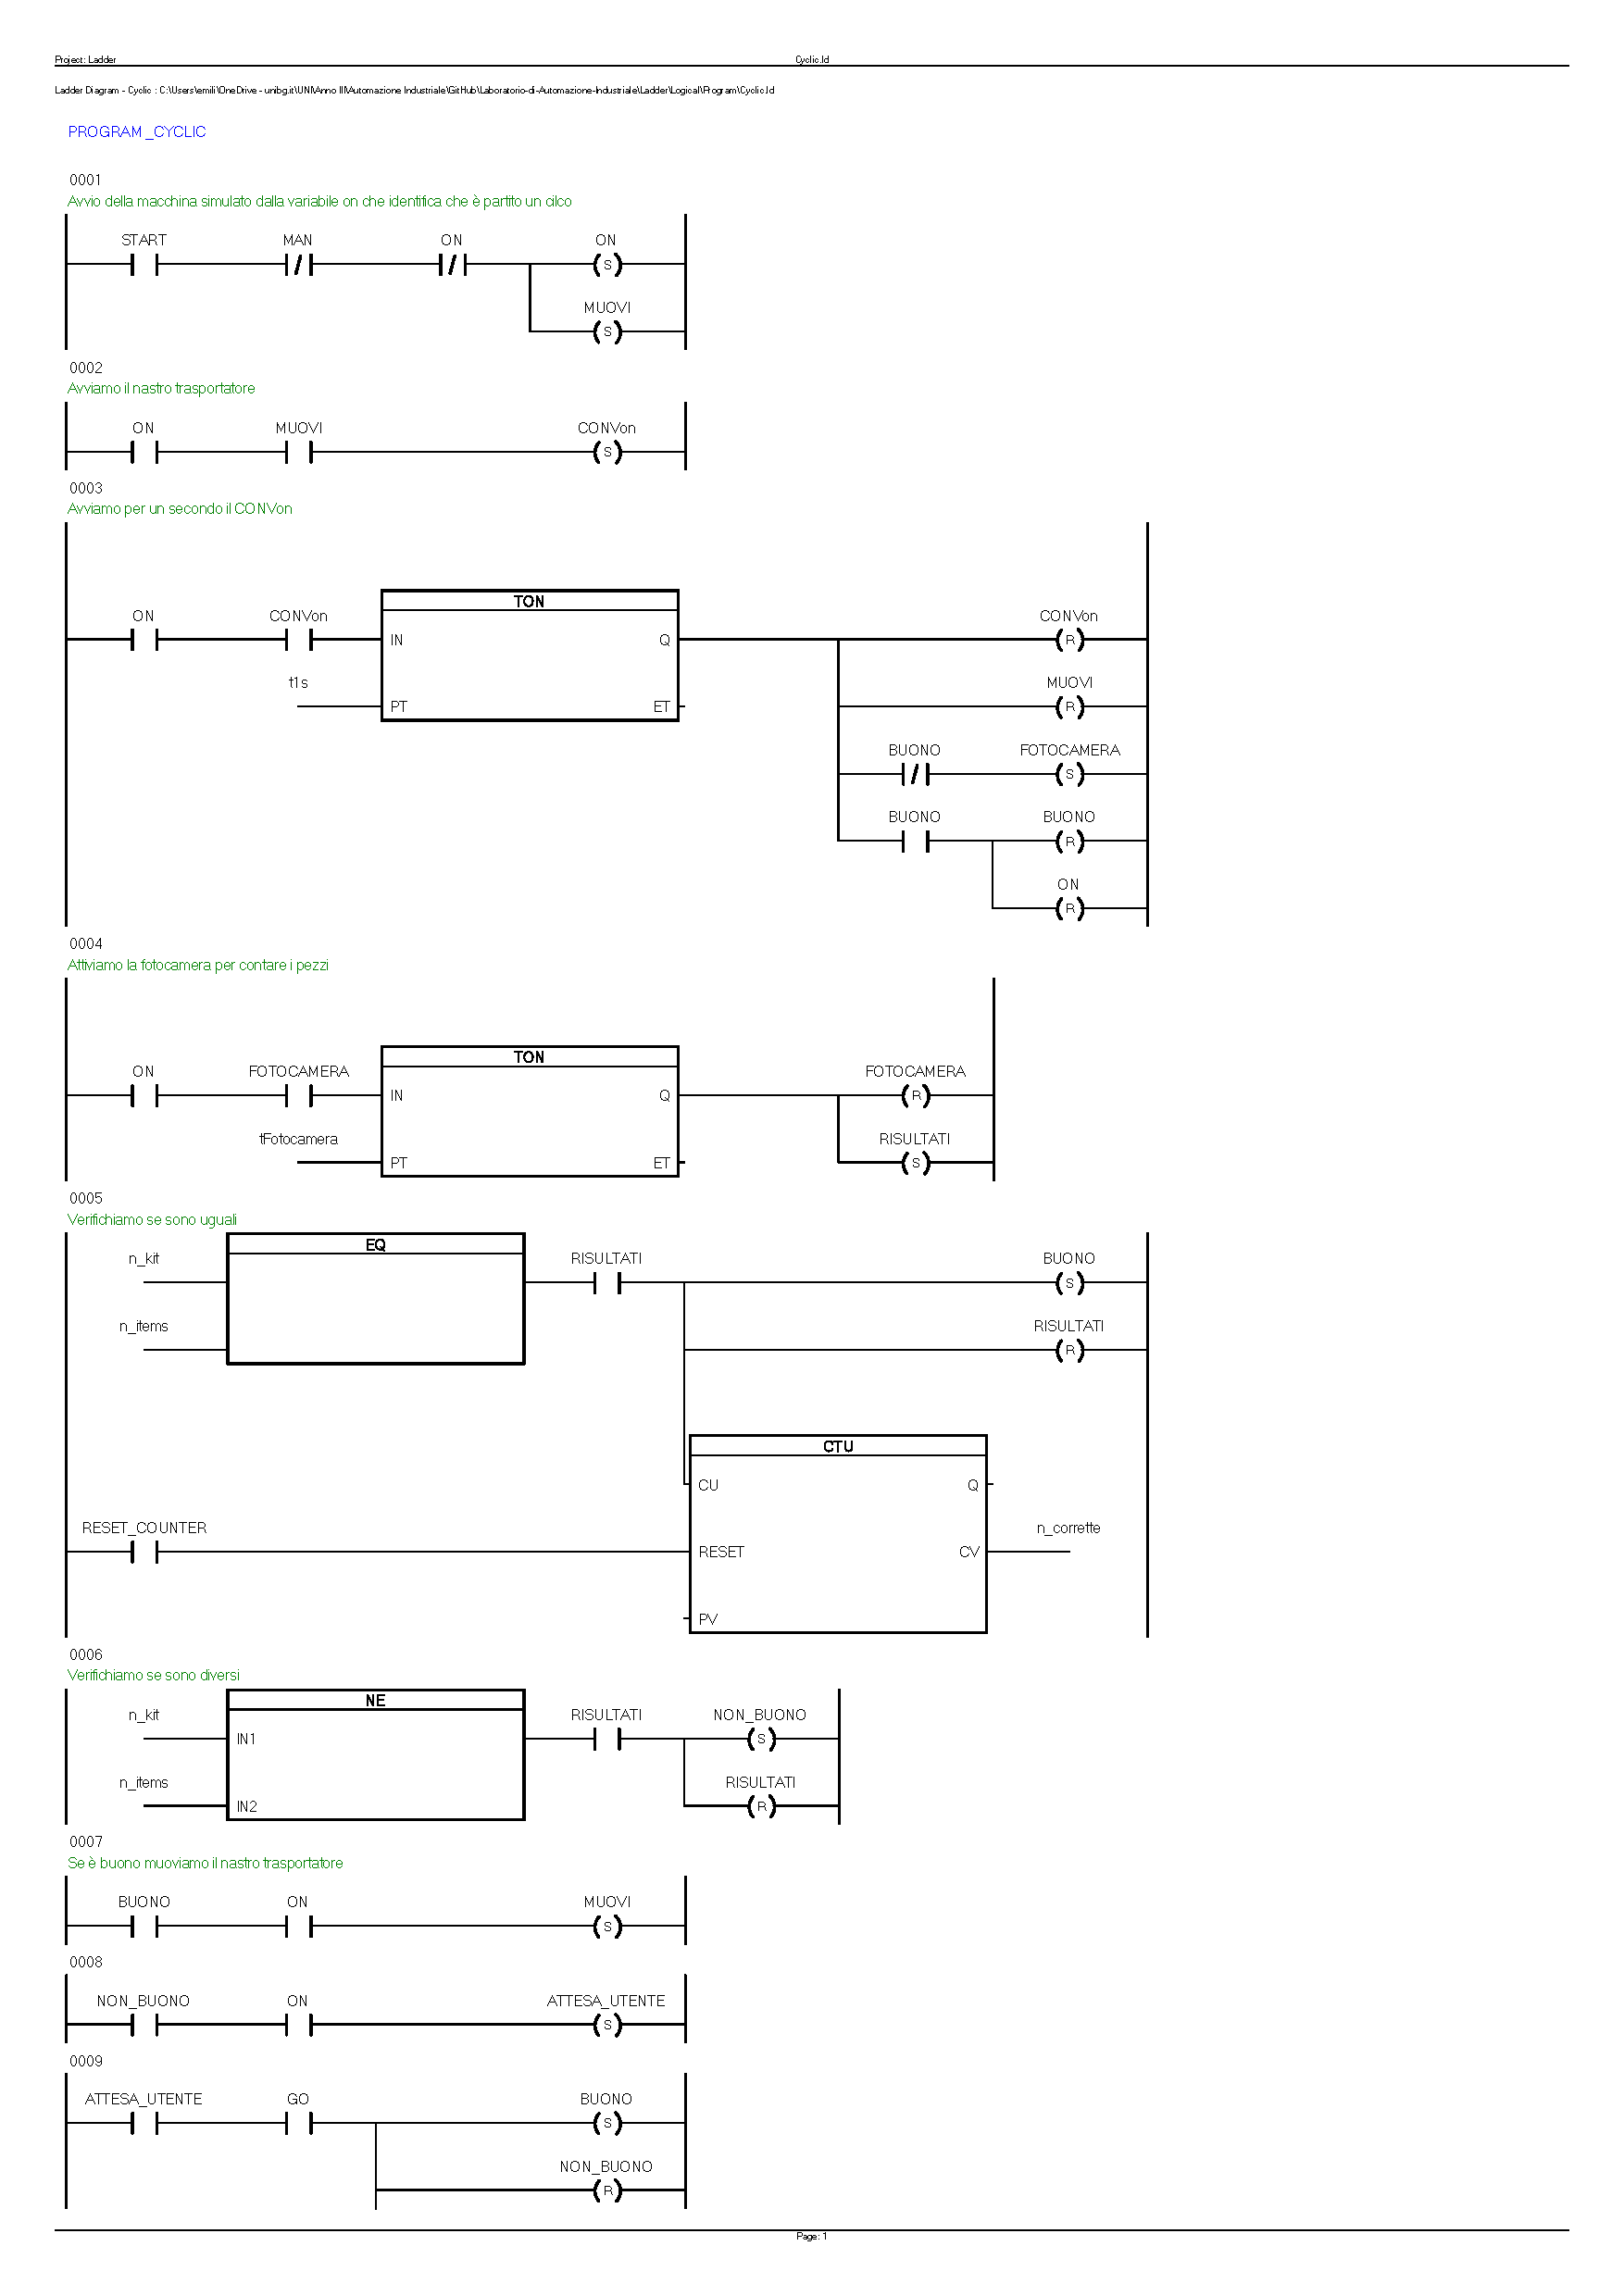
\includepdf[pages=-]{ProgrammaLadder.pdf}

\end{document}
